% homework/hw11x/hw11x.tex
% Year 7 - Extra Homework 11: How High Does It Bounce?
%
% Goes out alongside Homework 11 (homework/hw11, Sections A-F), due the same
% Friday. The teacher asked for "an easier extra homework packet that covers
% more decimal work mixed in with the science (and some angles)". So: Unit 4
% decimals, every one of them inside Science 3.4 Tides, 3.5 Energy and 3.6
% Changes in energy, and a light touch of Maths 5.1 (180 on a line, 360 round
% a point, the two steps).
%
% Same framing rule as hw03x-hw10x: nothing on the sheet says easy, basic,
% extra help, catch-up or revision. The cover states a fact, and it is true:
% there is nothing new to calculate here.
%
% Every method is printed as a frame, as in hw09x: column grids with the point
% column drawn and the zeros to write tinted orange; division frames with the
% point already up; tables whose scaffold fades (row 1 done, then partly
% printed, then empty).
%
% QUESTION NUMBERS ARE X1..X12. Homework 11 has Sections A-F and the two
% sheets go home together.
%
% Nothing untaught, and nothing from 3.7 (useful / wasted energy, percentages,
% "dissipated" are 3.7's and are kept out). Where every number comes from:
%   X1  Tide board readings 5.4, 4.4, 2.2, 1.2 m, four hours of one falling
%       tide (high 4 a.m., low 10 a.m.: 3.4's "6 hours from high to low"). The
%       two middle readings are a real tide's shape, to the nearest 0.2 m.
%   X2  Tidal range = high - low (3.4's write note). 16.3 m is the Bay of
%       Fundy, from the 3.4 deck's tidal range slide.
%   X3  3.4's Question 6 (average 5.0 m, range 2.0 m, deepest 6.0 m, NOT 7.0)
%       is row 1, worked; the other rows are new.
%   X4  The earth tide: Hanoi goes up and down about 30 cm, twice a day (3.4,
%       the earth tide slide), and nobody feels it because everything goes up
%       together (the slide's reveal).
%   X5  Balls dropped from 2 m: the tennis ball's 1.1 m is the 3.6 deck's
%       bouncing ball. The others are realistic (a bouncy ball keeps most of
%       its height, clay almost none); the egg is the deadpan one. At the
%       bounce some energy changes to sound and heat (3.6, slide 4).
%       HW 11's E3 uses a football bouncing to 1.3 m, so there is no football.
%   X6  The mean (3.1's lab), of three bounces.
%   X7  3.5's three numbers from the book (page 106): a floor of stairs
%       2 000 J, run 1 m 200 J, boil 1 litre 400 000 J. HW 11's D3 uses
%       4 floors, 45 m and 0.5 litre; this sheet does not.
%   X8  3.6's write note: thermal energy moves from hotter things to colder
%       things. Mr Bowen's coffee going cold is 3.5's story.
%   X9  The Earth turns 360 degrees in 24 hours (3.4's spinning-Earth model:
%       one press = 6 hours = a quarter turn).
%   X10 360 round a point (5.1). Three blades (the 3.6 wind farm), a fan, a
%       pizza (5.1's 8 slices, 45 degrees).
%   X11 180 on a straight line and the two steps (5.1).
%   X12 Everything at once.
%
% FRENCH COPY. \fr{...} prints a grey French line under the English and
% \frin{...} a short French gloss in brackets. Both are EMPTY in the English
% copy. The English key words stay English inside the French lines, in blue.
% Numbers keep the English decimal point, as the class does.
%
% House style is shared: see homework/hw-style.tex. Method: the new-homework
% skill. Source is pure ASCII on purpose: French accents are written \'e etc.
%
% Build:  pwsh .claude/skills/new-homework/scripts/build-hw.ps1 hw11x -French

\documentclass[12pt,a4paper]{article}

% -- Answer key switch -------------------------------------------------------
\newif\ifkey
\ifdefined\TEACHER\keytrue\else
  \keyfalse        % \keyfalse = student copy   |   \keytrue = teacher copy
\fi

% -- Language switch ---------------------------------------------------------
\newif\iffr
\ifdefined\FRENCH\frtrue\fi

% -- House style -------------------------------------------------------------
% homework/hw-style.tex
% Shared house style for every Year 7 homework packet. \input this from the
% packet file, right after \documentclass and the answer-key switch.
%
% Do not fork this file per packet. If a packet needs a different look, the
% question is whether every packet should have it.
%
% The choices here are deliberate and were arrived at by printing and looking:
%   * No solid dark banners. Every header is a light tint with a coloured spine
%     on the left, so colour reads clearly without flooding a school printer.
%   * No marks and no mark totals. These are practice, not exam papers.
%   * Lato at 12pt with open leading, plus mathastext so inline maths is Lato
%     too. Without mathastext every "-6 + 4" is Computer Modern serif and the
%     sheet looks half-typeset.
%   * Writing lines are spaced for Year 7 handwriting, not adult margin notes.
%   * Pages fill. \needspace is redefined below so a heading no longer drags
%     the page break up to itself, and every heading is glued to the box under
%     it. Packets built before 2026-09-30 were laid out under the old rules and
%     will reflow if rebuilt -- re-read every page if you rebuild one.
%
% Provides: \wlines \blank \tickbox \sep \qmk-free marks (none) \hwsection
% \qhead \expr, the workspace box, and the remember / wordhelp / activity /
% yourturn coloured boxes. Palette matches the lesson decks exactly.

% -- Packages ----------------------------------------------------------------
\usepackage[T1]{fontenc}
\usepackage[utf8]{inputenc}
\usepackage[default]{lato}
\usepackage[a4paper,top=1.7cm,bottom=1.7cm,left=2.0cm,right=2.0cm,headheight=15pt]{geometry}
\usepackage{amsmath,amssymb}
\usepackage{xcolor}
\usepackage[most]{tcolorbox}
\usepackage{enumitem}
\usepackage{tikz}
\usetikzlibrary{arrows.meta}
\usepackage{array}
\usepackage{tabularx}
\usepackage{fancyhdr}
\usepackage{multicol}
\usepackage{needspace}
\usepackage{graphicx}

% Make maths use Lato too. Without this, every "-6 + 4" on the page is set in
% Computer Modern serif and the sheet looks half-typeset. Must come last.
\usepackage[italic]{mathastext}

% -- \needspace, without the hole it used to leave ----------------------------
% needspace.sty writes "\vskip 0pt plus X \penalty-100" in front of every
% heading. A page that ends anywhere else is underfull with no stretch, so TeX
% scores it b=10000; a page that ends AT a heading gets that X of stretch and a
% finite badness, and wins. So any heading in roughly the bottom half of a page
% claimed the break, and the question under it moved over whole, leaving a hole
% the size of the question. \tracingpages showed it exactly (b=4531 at the
% heading, b=10000 at every later break) while building homework/q1rev, and it
% is where the half-empty pages in HW 1-8 came from.
% This keeps only the \penalty9999, which still refuses to put a heading in the
% last X of a page. Keeping a heading WITH the box under it is \nobreak's job
% now -- see \hwsection and \qhead below.
\makeatletter
\renewcommand{\needspace}[1]{\begingroup\setlength{\dimen@}{#1}%
  \vskip\dimen@\penalty9999\vskip-\dimen@\endgroup}
\makeatother

\linespread{1.06}\selectfont

% -- The Learner's Book palette (same hex values as the lesson decks) ---------
\definecolor{cbteal}{HTML}{0087A8}
\definecolor{cbpurple}{HTML}{5C2483}
\definecolor{cborange}{HTML}{C25E12}
\definecolor{cbgreen}{HTML}{4A8B23}
\definecolor{cbred}{HTML}{C8102E}
\definecolor{cbblue}{HTML}{1A5FA8}
\definecolor{rulegray}{HTML}{9AA5AD}

% -- Answer lines and blanks -------------------------------------------------
% \wlines{n} draws n ruled writing lines, spaced wide enough for Year 7
% handwriting rather than for an adult with a fine pen.
\makeatletter
\newcommand{\wlines}[1]{%
  \par\vspace{0.75em}%
  \@tempcnta=0\relax
  \@whilenum\@tempcnta<#1\do{%
    \hbox to \linewidth{\color{rulegray}\leaders\hrule height 0.5pt\hfill}%
    \vspace{1.5em}%
    \advance\@tempcnta by 1\relax}%
  \par\vspace{-0.8em}%
}
\makeatother

% \blank[width] is an inline gap to write a short answer in.
\newcommand{\blank}[1][2.6cm]{\underline{\hspace{#1}}}

% A boxed space for showing working.
\newtcolorbox{workspace}[1][3.4cm]{%
  colback=white, colframe=rulegray, boxrule=0.5pt, arc=5pt,
  height=#1, left=6pt, right=6pt, top=4pt, bottom=4pt,
  before skip=9pt, after skip=11pt}

% An empty tick box.
\newcommand{\tickbox}{\fbox{\rule{0pt}{1.15em}\rule{1.15em}{0pt}}}

% A middot separator.
\newcommand{\sep}{\,\textperiodcentered\,}

% -- Section and question headings -------------------------------------------
% Light tint plus a fat coloured spine on the left. No solid dark banner: the
% colour reads clearly but barely costs the printer anything.
% needspace keeps a heading out of the last few lines of a page. The \nobreak
% after it keeps it with whatever comes next: a remember or word-help box that
% does not fit takes its heading over with it, instead of leaving the heading
% alone at the foot of the page. (The old needspace did that by accident, and
% left a hole every time; see above.)
\newcommand{\hwsection}[2][cbteal]{%
  \needspace{8\baselineskip}%
  \par\vspace{13pt}%
  \noindent
  \begin{tcolorbox}[enhanced, nobeforeafter, width=\textwidth,
      colback=#1!7, colframe=#1!7, arc=5pt,
      borderline west={5pt}{0pt}{#1},
      left=14pt, right=10pt, top=7pt, bottom=7pt]
    {\large\bfseries\color{#1}#2}
  \end{tcolorbox}%
  \par\nobreak\vspace{9pt}}

% \qhead[colour]{A2}{Moving along the line} -- a question heading.
\newcommand{\qhead}[3][cbteal]{%
  \needspace{6\baselineskip}%
  \par\vspace{11pt}%
  \noindent{\large\bfseries\color{#1}#2}\quad{\large\bfseries #3}\par\nobreak\vspace{4pt}}

% -- Coloured boxes ----------------------------------------------------------
% Shared look: rounded, light fill, coloured rule, coloured title text on a
% pale title strip rather than a dark one.
% NOT breakable. A breakable box that cannot fit its first lines forces its own
% page break, and \nobreak cannot stop a forced break -- so the heading above
% it was left alone at the foot of the page (tested: it happens with \nobreak
% in place). Unbreakable, the page builder moves heading and box together.
% These boxes are a few lines each; none needs to split.
\tcbset{hwbox/.style={
  enhanced, arc=6pt, boxrule=1pt,
  left=11pt, right=11pt, top=8pt, bottom=8pt,
  fonttitle=\bfseries, attach boxed title to top left={xshift=12pt, yshift=-8pt},
  boxed title style={arc=4pt, boxrule=1pt, left=7pt, right=7pt, top=2pt, bottom=2pt},
  top=13pt}}

% Orange: things to remember. Matches the deck's "Write This Down".
\newtcolorbox{remember}[1][Remember from the lesson]{hwbox,
  colback=cborange!6, colframe=cborange, coltitle=cborange,
  colbacktitle=white, title={#1}}

% Blue: English help. The barrier in this class is the wording, not the maths.
\newtcolorbox{wordhelp}[1][Word help]{hwbox,
  colback=cbblue!6, colframe=cbblue, coltitle=cbblue,
  colbacktitle=white, title={#1}}

% Purple: an activity or instruction.
\newtcolorbox{activity}[1][How to do this homework]{hwbox,
  colback=cbpurple!6, colframe=cbpurple, coltitle=cbpurple,
  colbacktitle=white, title={#1}}

% Green: your turn / a friendly nudge.
\newtcolorbox{yourturn}[1][Your turn]{hwbox,
  colback=cbgreen!7, colframe=cbgreen, coltitle=cbgreen!75!black,
  colbacktitle=white, title={#1}}

% -- Shorthands --------------------------------------------------------------
\newcommand{\dC}{\,^{\circ}\mathrm{C}}          % use inside maths: $-8\dC$
\newcommand{\key}[1]{{\color{cborange}\textbf{#1}}}
\newcommand{\eng}[1]{{\color{cbblue}\textbf{#1}}}

\setlist[enumerate]{itemsep=8pt, topsep=5pt, leftmargin=*}
\setlist[itemize]{itemsep=4pt, topsep=4pt, leftmargin=*}
\renewcommand{\arraystretch}{1.45}

% -- An expression the student is asked to work from -------------------------
\newcommand{\expr}[1]{%
  \tcbox[on line, colback=cbgreen!10, colframe=cbgreen!55, boxrule=1pt, arc=4pt,
         left=9pt, right=9pt, top=4pt, bottom=4pt]{\large\bfseries $#1$}}

% -- Running head and foot ---------------------------------------------------
% The packet overrides \fancyhead[L] with its own title.
\pagestyle{fancy}
\fancyhf{}
\fancyhead[L]{\small\color{black!55}Year 7\sep Homework}
\fancyhead[R]{\small\color{black!55}Name: \blank[3.4cm]}
\fancyfoot[C]{\small\color{black!55}Page \thepage}
\renewcommand{\headrulewidth}{0pt}
\renewcommand{\headrule}{\vspace{2pt}\hbox to\headwidth{\color{cbteal!45}\leaders\hrule height 1.2pt\hfill}}


\usetikzlibrary{calc}

% -- French support lines ----------------------------------------------------
% \fr{...}  a French line of its own, grey and italic, under the English.
% \frin{...} a French gloss in brackets, inline -- for table cells and labels.
% \fq{...}  French quotation marks.
% Both start with \unskip: the line break before \fr is a space, and in the
% English copy it would otherwise sit at the end of the line and move a break.
\newcommand{\fr}[1]{\unskip\iffr\par\nobreak\vspace{1pt}\noindent{\small\itshape\color{black!60}#1}\par\fi}
\newcommand{\frin}[1]{\unskip\iffr\ {\small\itshape\color{black!60}(#1)}\fi}
\newcommand{\fq}[1]{\guillemotleft\,#1\,\guillemotright}
% \frl{english}{french}: a size that is bigger in the French copy.
\newcommand{\frl}[2]{\iffr#2\else#1\fi}

% The X1 tide board's metre. Set here: a conditional cannot go inside TikZ's
% options.
\iffr\def\boardy{1.0cm}\else\def\boardy{1.12cm}\fi

% -- Per-packet running head -------------------------------------------------
\iffr
  \fancyhead[L]{\small\color{black!55}Year 7\sep Extra Homework 11\sep English /
    Fran\c{c}ais}
\else
  \fancyhead[L]{\small\color{black!55}Year 7\sep Extra Homework 11}
\fi

% -- Writing lines that will not be split from their question ----------------
% In a minipage, so inside a list the lines start at the item's indent, and
% after \nobreak, so they cannot go over a page break without the question.
\newcommand{\qlines}[1]{\par\nobreak
  \noindent\begin{minipage}{\linewidth}\wlines{#1}\end{minipage}\par}

% -- A box to write one digit or sign in -------------------------------------
\newcommand{\nbox}{\ \fbox{\rule{0pt}{1.05em}\rule{1.0em}{0pt}}\ }
% A box with no space round it, tinted: write a 0 here.
\newcommand{\zb}{\fcolorbox{cborange}{cborange!14}{\rule{0pt}{0.95em}\rule{0.75em}{0pt}}}

% -- An answer blank on a line of its own, right-aligned ---------------------
\newcommand{\ansline}[1][4.4cm]{\par\nobreak\vspace{2pt}\hspace*{\fill}\blank[#1]\par}

% -- Columns -----------------------------------------------------------------
\newcolumntype{L}{>{\raggedright\arraybackslash}X}
\newcolumntype{C}[1]{>{\centering\arraybackslash}p{#1}}
% \leavevmode, so a cell that starts with a \color is not dropped a line.
\newcolumntype{P}[1]{>{\leavevmode\raggedright\arraybackslash}p{#1}}
% The word-help term column.
\newcolumntype{W}[1]{>{\leavevmode\raggedright\bfseries\color{cbblue}}p{#1}}

% -- A table row tall enough to write in -------------------------------------
\newcommand{\tall}{\rule[-0.6em]{0pt}{1.9em}}

% -- More room in the French copy --------------------------------------------
% Same scheme as hw09x and hw10x: looser leading, taller table rows, working
% boxes a third taller and wider writing lines in the French copy only. The
% English copy is untouched by all of this.
\iffr
  \linespread{1.10}\selectfont
  \renewcommand{\tall}{\rule[-0.8em]{0pt}{2.4em}}
  \renewtcolorbox{workspace}[1][3.4cm]{%
    colback=white, colframe=rulegray, boxrule=0.5pt, arc=5pt,
    height={1.33\dimexpr #1\relax}, left=6pt, right=6pt, top=4pt, bottom=4pt,
    before skip=9pt, after skip=11pt}
  \makeatletter
  \renewcommand{\wlines}[1]{%
    \par\vspace{0.75em}%
    \@tempcnta=0\relax
    \@whilenum\@tempcnta<#1\do{%
      \hbox to \linewidth{\color{rulegray}\leaders\hrule height 0.5pt\hfill}%
      \vspace{1.9em}%
      \advance\@tempcnta by 1\relax}%
    \par\vspace{-0.8em}}
  \makeatother
\fi

% ---------------------------------------------------------------------------
% COLUMN GRID. \colgrid{op}{row 1}{row 2}{answer row}
% Each row is four entries: tens, ones, tenths, hundredths. The point column
% sits between ones and tenths and is printed on every row, so it cannot move.
% An entry is a digit, nothing, z (an orange box: write a 0 here) or Z (an
% orange box with the 0 already written -- for a worked example).
% \hgrid is the same with hundreds, tens, ones, tenths (for 180.0 - 32.5), and
% \colgridiii adds a third number row (three bounces to add for a mean).
% ---------------------------------------------------------------------------
\def\zz{z}
\def\ZZ{Z}
\def\pt{.}
\newcommand{\gcell}[4][black]{%
  \edef\gcE{#4}%
  \ifx\gcE\zz
    \filldraw[fill=cborange!14, draw=cborange!80, line width=0.8pt]
      (#2,#3) rectangle ++(0.72,0.78);
  \else\ifx\gcE\ZZ
    \filldraw[fill=cborange!14, draw=cborange!80, line width=0.8pt]
      (#2,#3) rectangle ++(0.72,0.78);
    \node[font=\large\bfseries, text=cborange] at (#2+0.36,#3+0.39) {0};
  \else
    \draw[rulegray, line width=0.6pt] (#2,#3) rectangle ++(0.72,0.78);
    \node[font=\large, text=#1] at (#2+0.36,#3+0.39) {\gcE};
  \fi\fi}
\newcommand{\colgrid}[4]{%
  \begin{tikzpicture}[x=1cm, y=1cm, baseline=(current bounding box.north)]
    \foreach \d [count=\i] in {#2}{%
      \pgfmathsetmacro\xx{(\i-1)*0.72+(\i>2)*0.30}\gcell{\xx}{1.75}{\d}}
    \foreach \d [count=\i] in {#3}{%
      \pgfmathsetmacro\xx{(\i-1)*0.72+(\i>2)*0.30}\gcell{\xx}{0.85}{\d}}
    \foreach \d [count=\i] in {#4}{%
      \pgfmathsetmacro\xx{(\i-1)*0.72+(\i>2)*0.30}\gcell[cbteal]{\xx}{-0.25}{\d}}
    \foreach \y in {1.75,0.85,-0.25}{\fill (1.59,\y+0.13) circle (0.06);}
    \node[font=\Large] at (-0.42,1.24) {$#1$};
    \draw[line width=1.2pt] (-0.75,0.72) -- (3.18,0.72);
  \end{tikzpicture}}
\newcommand{\hgrid}[4]{%
  \begin{tikzpicture}[x=1cm, y=1cm, baseline=(current bounding box.north)]
    \foreach \d [count=\i] in {#2}{%
      \pgfmathsetmacro\xx{(\i-1)*0.72+(\i>3)*0.30}\gcell{\xx}{1.75}{\d}}
    \foreach \d [count=\i] in {#3}{%
      \pgfmathsetmacro\xx{(\i-1)*0.72+(\i>3)*0.30}\gcell{\xx}{0.85}{\d}}
    \foreach \d [count=\i] in {#4}{%
      \pgfmathsetmacro\xx{(\i-1)*0.72+(\i>3)*0.30}\gcell[cbteal]{\xx}{-0.25}{\d}}
    \foreach \y in {1.75,0.85,-0.25}{\fill (2.31,\y+0.13) circle (0.06);}
    \node[font=\Large] at (-0.42,1.24) {$#1$};
    \draw[line width=1.2pt] (-0.75,0.72) -- (3.18,0.72);
  \end{tikzpicture}}
\newcommand{\colgridiii}[4]{%
  \begin{tikzpicture}[x=1cm, y=1cm, baseline=(current bounding box.north)]
    \foreach \d [count=\i] in {#1}{%
      \pgfmathsetmacro\xx{(\i-1)*0.72+(\i>2)*0.30}\gcell{\xx}{2.65}{\d}}
    \foreach \d [count=\i] in {#2}{%
      \pgfmathsetmacro\xx{(\i-1)*0.72+(\i>2)*0.30}\gcell{\xx}{1.75}{\d}}
    \foreach \d [count=\i] in {#3}{%
      \pgfmathsetmacro\xx{(\i-1)*0.72+(\i>2)*0.30}\gcell{\xx}{0.85}{\d}}
    \foreach \d [count=\i] in {#4}{%
      \pgfmathsetmacro\xx{(\i-1)*0.72+(\i>2)*0.30}\gcell[cbteal]{\xx}{-0.25}{\d}}
    \foreach \y in {2.65,1.75,0.85,-0.25}{\fill (1.59,\y+0.13) circle (0.06);}
    \node[font=\Large] at (-0.42,1.24) {$+$};
    \draw[line width=1.2pt] (-0.75,0.72) -- (3.18,0.72);
  \end{tikzpicture}}

% ---------------------------------------------------------------------------
% DIVISION FRAME. \bus{divisor}{dividend}
% The dividend is a list of entries: a digit, . (the point) or z (an orange
% box: write a 0 here and keep dividing). Above every digit is an empty box for
% the answer; above the point the point is already printed: the point goes
% straight up, drawn. An entry b is an empty box in the number itself: the
% student writes the total there first (X6(b)).
% ---------------------------------------------------------------------------
\def\bb{b}
\newcommand{\bus}[2]{%
  \begin{tikzpicture}[x=1cm, y=1cm, baseline=(current bounding box.north)]
    \draw[line width=1.2pt] (-0.20,0.86) -- (0,0.86);
    \foreach \d [count=\i] in {#2}{%
      \pgfmathsetmacro{\xx}{(\i-1)*0.66}%
      \edef\gcE{\d}%
      \draw[line width=1.2pt] (\xx,0.86) -- (\xx+0.66,0.86);
      \ifx\gcE\pt
        \fill (\xx+0.33,0.12) circle (0.06);
        \fill (\xx+0.33,1.10) circle (0.06);
      \else
        \draw[rulegray, line width=0.6pt] (\xx+0.04,0.98) rectangle ++(0.58,0.74);
        \ifx\gcE\zz
          \filldraw[fill=cborange!14, draw=cborange!80, line width=0.8pt]
            (\xx+0.04,0.04) rectangle ++(0.58,0.74);
        \else\ifx\gcE\bb
          \draw[rulegray, line width=0.6pt] (\xx+0.04,0.04) rectangle ++(0.58,0.74);
        \else
          \node[font=\large] at (\xx+0.33,0.41) {\gcE};
        \fi\fi
      \fi}
    \draw[line width=1.2pt] (-0.20,-0.02) .. controls (-0.06,0.42) .. (-0.20,0.86);
    \node[font=\large] at (-0.55,0.41) {#1};
  \end{tikzpicture}}

% -- X10: a circle cut into n equal parts, one angle marked "?" ---------------
% \spokes{n}{start angle}
\newcommand{\spokes}[2]{%
  \begin{tikzpicture}[baseline=(current bounding box.north)]
    \draw[cbteal, line width=1pt, fill=cbteal!6] (0,0) circle (0.78);
    \foreach \k in {1,...,#1}
      \draw[black!75, line width=1.1pt] (0,0) -- ({#2+(\k-1)*360/#1}:0.78);
    \draw[cborange, line width=1pt] ({#2}:0.32) arc ({#2}:{#2+360/#1}:0.32);
    \node[font=\small\bfseries, text=cborange] at ({#2+180/#1}:0.52) {?};
    \fill[black] (0,0) circle (1.6pt);
  \end{tikzpicture}}

\begin{document}

% ===========================================================================
% COVER BLOCK
% ===========================================================================
\thispagestyle{fancy}

\begin{tcolorbox}[enhanced, colback=cbgreen!8, colframe=cbgreen!8, arc=7pt,
                  borderline west={6pt}{0pt}{cbgreen},
                  left=18pt, right=14pt, top=11pt, bottom=11pt]
  {\color{cbgreen!75!black}\bfseries YEAR 7\sep SCIENCE 3.4--3.6\sep MATHS 5.1\sep
  EXTRA HOMEWORK 11}\\[6pt]
  {\color{cbgreen!70!black}\Huge\bfseries How High Does It Bounce?}\\[10pt]
  {\color{black!70}Tides\sep bouncing balls\sep joules\sep a cooling coffee\sep
  angles --- all in decimals}
  \iffr\\[4pt]{\small\itshape\color{black!60}\`A quelle hauteur rebondit-elle~?
  Les mar\'ees, les balles qui rebondissent, les joules, un caf\'e qui refroidit et
  les angles --- avec des nombres d\'ecimaux}\fi
\end{tcolorbox}

\vspace{6pt}
\noindent
\begin{tabularx}{\textwidth}{@{}X X@{}}
  \textbf{Name:} \blank[5.6cm] & \textbf{Class:} \blank[5.6cm] \\
  \textbf{Date given:} \blank[4.6cm] &
  \textbf{Date due:} {\color{cbred}\bfseries Friday 6 November 2026} \\
\end{tabularx}

\vspace{4pt}
\begin{activity}[Why this sheet exists]
  There is \key{nothing new to calculate} here. Every number is a Unit 4 decimal,
  and every question is this week's science: the tides, energy, and a ball that
  will not bounce back to where it started.
  \fr{Ici, il n'y a \textbf{rien de nouveau \`a calculer}. Chaque nombre est un
  d\'ecimal de l'unit\'e 4, et chaque question vient des sciences de la semaine~:
  les mar\'ees, l'\'energie, et une balle qui ne remonte jamais aussi haut. En
  anglais, la virgule s'appelle \eng{the point} et s'\'ecrit avec un point~: 3.25.}

  \medskip
  The steps are printed as \key{boxes}. Fill the boxes --- that \emph{is} the method.
  An \key{orange box} means: write a \key{0} here.
  \fr{Les \'etapes sont d\'ej\`a dessin\'ees~: remplir les cases, c'est appliquer la
  m\'ethode. Une case orange veut dire~: \'ecris un 0 ici.}

  \medskip
  \eng{No calculator.} \; Answer in \key{full sentences} when it says so.
  \frin{Calculatrice interdite. R\'eponds par des phrases compl\`etes, en anglais,
  quand on te le demande.}
\end{activity}

% ===========================================================================
% PART 1 -- TIDES IN DECIMALS
% ===========================================================================
\hwsection[cbgreen]{Part 1 \textperiodcentered\ Tides in decimals\frin{Les mar\'ees en
d\'ecimaux}}

% -- X1 ---------------------------------------------------------------------
% The way in. Four readings of one falling tide, every one on a tick. Two are
% one tick above a whole metre, two are two ticks above. Ordering them is easy
% on purpose: the board does it.
\qhead[cbgreen]{X1}{Read the tide board}

\noindent\begin{minipage}{\textwidth}
\noindent\begin{minipage}[c]{0.30\textwidth}\centering
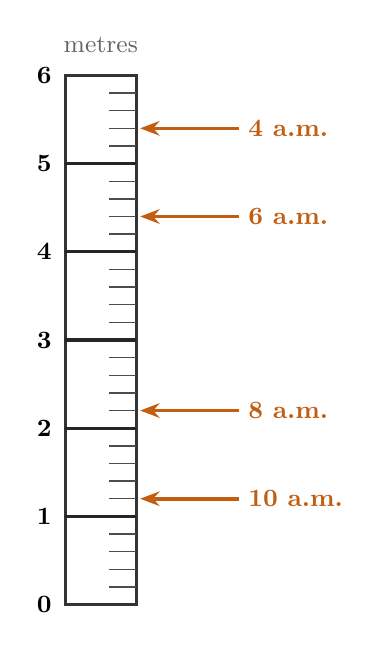
\begin{tikzpicture}[x=1cm, y=\boardy]
  % the board
  \fill[white] (0,0) rectangle (0.9,6);
  \draw[black!80, line width=1pt] (0,0) rectangle (0.9,6);
  % 0.2 m ticks from the right edge; whole metres right across
  \foreach \k in {1,...,29}{\draw[black!70, line width=0.5pt] (0.9,\k*0.2) -- (0.55,\k*0.2);}
  \foreach \m in {1,...,5}{\draw[black!85, line width=1.1pt] (0,\m) -- (0.9,\m);}
  \foreach \m in {0,...,6}{\node[left, font=\small\bfseries] at (-0.05,\m) {\m};}
  \node[font=\small, text=black!60] at (0.45,6.35) {metres};
  % the four readings
  \foreach \d/\t in {5.4/4 a.m., 4.4/6 a.m., 2.2/8 a.m., 1.2/10 a.m.}{
    \draw[cborange, line width=1.3pt, -{Stealth[length=7pt]}] (2.2,\d) -- (0.95,\d);
    \node[right, font=\small\bfseries, text=cborange] at (2.2,\d) {\t};}
\end{tikzpicture}
\end{minipage}\hfill
\begin{minipage}[c]{0.66\textwidth}
\begin{wordhelp}[Word help]
  \renewcommand{\arraystretch}{1.15}%
  \begin{tabularx}{\linewidth}{@{}W{2.3cm}X@{}}
    tide board & a tall ruler on the harbour wall. It shows the \textbf{depth} of
      the sea. \frin{une \'echelle de mar\'ee~: une grande r\`egle sur le mur du
      port} \\
    depth & how deep the water is \frin{la profondeur} \\
  \end{tabularx}
\end{wordhelp}

\vspace{2pt}
Mr Bowen looks at the tide board every 2 hours. Every small line is \key{0.2 m}.
Count in 0.2s: \; 5, \,5.2, \,5.4.
\fr{Mr Bowen regarde l'\'echelle de mar\'ee toutes les 2 heures. Chaque petite
graduation vaut 0.2 m. Compte de 0.2 en 0.2~: 5, 5.2, 5.4.}

\vspace{6pt}
\noindent\textbf{(a)} Write the depth at each time.
\fr{(a) \'Ecris la profondeur \`a chaque heure.}

\vspace{4pt}
{\setlength{\tabcolsep}{4pt}%
\begin{tabular}{|l|C{1.45cm}|C{1.45cm}|C{1.45cm}|C{1.45cm}|}
  \hline
  \textbf{Time} & 4 a.m. & 6 a.m. & 8 a.m. & 10 a.m. \\ \hline
  \textbf{Depth} (m) \tall & & & & \\ \hline
\end{tabular}}

\vspace{8pt}
\noindent\textbf{(b)} Which time was \textbf{high tide}? \frin{mar\'ee haute} \hfill
\blank[2.2cm] \\[6pt]
\textbf{(c)} Which time was \textbf{low tide}? \frin{mar\'ee basse} \hfill
\blank[2.2cm]
\end{minipage}
\end{minipage}

% -- X2 ---------------------------------------------------------------------
% Tidal range = high - low, the 3.4 write note. (a) is X1's high and low,
% worked. (b) and (c) need a 0 written; (d) is the Bay of Fundy from the deck.
\qhead[cbgreen]{X2}{The tidal range}

\begin{remember}[Tidal range, from Science 3.4]
  \key{Tidal range}: the difference in depth between high tide and low tide.
  \quad It is a \key{subtraction}: \; high tide $-$ low tide.
  \fr{Le marnage (\eng{tidal range})~: la diff\'erence de profondeur entre la mar\'ee
  haute et la mar\'ee basse. C'est une soustraction~: mar\'ee haute $-$ mar\'ee
  basse.}
\end{remember}

\noindent\begin{minipage}{\textwidth}
Write a 0 in every orange box. Then subtract. \textbf{(a)} is done for you.
\fr{\'Ecris un 0 dans chaque case orange, puis soustrais. Le (a) est fait pour toi.}

\vspace{8pt}
\noindent
\begin{minipage}[t]{0.32\textwidth}\centering
  \textbf{(a)} Mr Bowen's harbour \frin{le port de Mr Bowen}\\
  high $5.4$ m, \, low $1.2$ m\par\vspace{6pt}
  \colgrid{-}{,5,4,}{,1,2,}{,4,2,}\par\vspace{4pt}
  Range: \textbf{4.2 m}
\end{minipage}\hfill
\begin{minipage}[t]{0.32\textwidth}\centering
  \textbf{(b)} Another harbour \frin{un autre port}\\
  high $3.75$ m, \, low $0.9$ m\par\vspace{6pt}
  \colgrid{-}{,3,7,5}{,0,9,z}{,,,}\par\vspace{4pt}
  Range: \blank[1.6cm] m
\end{minipage}\hfill
\begin{minipage}[t]{0.32\textwidth}\centering
  \textbf{(c)} A third harbour \frin{un troisi\`eme port}\\
  high $6.1$ m, \, low $2.35$ m\par\vspace{6pt}
  \colgrid{-}{,6,1,z}{,2,3,5}{,,,}\par\vspace{4pt}
  Range: \blank[1.6cm] m
\end{minipage}
\end{minipage}

\vspace{10pt}
\noindent\begin{minipage}{\textwidth}
\noindent\begin{minipage}[c]{0.60\textwidth}
\textbf{(d)} The Bay of Fundy in Canada has the biggest tides in the world. Its
tidal range is \textbf{16.3 m}. How much bigger is that than the range at Mr Bowen's
harbour (4.2 m)?
\fr{(d) La baie de Fundy, au Canada, a les plus grandes mar\'ees du monde~: son
marnage est de 16.3 m. De combien est-il plus grand (\eng{how much bigger}) que celui
du port de Mr Bowen (4.2 m)~?}

\vspace{4pt}
{\small\color{cbblue}\textbf{how much bigger?} = the difference = subtract}
\frin{de combien plus grand~? = la diff\'erence = soustraire}

\vspace{6pt}
Line up the points in the grid yourself. \frin{Place toi-m\^eme les nombres dans la
grille, virgule sous virgule.}

\vspace{6pt}
Answer: \blank[2.0cm] m
\end{minipage}\hfill
\begin{minipage}[c]{0.36\textwidth}\centering
  \colgrid{-}{,,,}{,,,}{,,,}
\end{minipage}
\end{minipage}

% -- X3 ---------------------------------------------------------------------
% 3.4's Question 6, the trap: average 5.0 m and range 2.0 m do NOT make 7.0 m.
% Row 1 is the deck's own numbers, worked. Row 2 has its sums printed, rows 3
% and 4 are empty. (b) is the trap, made by Mr Bowen on row 2.
\qhead[cbgreen]{X3}{Half above, half below}

\begin{remember}[The deepest water]
  \noindent\begin{minipage}[c]{0.66\linewidth}
  The water goes \key{half the range above} the average depth, and \key{half the
  range below} it. \\[3pt]
  Average $5.0$ m, \, range $2.0$ m: \; half the range is $1.0$ m. \\
  Deepest: $5.0 + 1.0 = \mathbf{6.0}$ m. \; Not $7.0$ m!
  \fr{L'eau monte de la moiti\'e du marnage au-dessus de la profondeur moyenne
  (\eng{average depth}), et descend de la moiti\'e en dessous. Le plus profond~: 6.0
  m, pas 7.0 m~!}
  \end{minipage}\hfill
  \begin{minipage}[c]{0.30\linewidth}\centering
  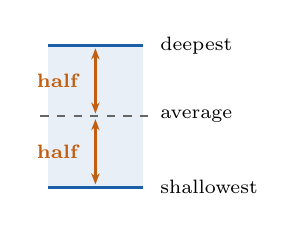
\begin{tikzpicture}[x=1cm, y=0.9cm]
    \fill[cbblue!10] (0,0) rectangle (1.2,2);
    \draw[cbblue, line width=1pt] (0,2) -- (1.2,2);
    \draw[cbblue, line width=1pt] (0,0) -- (1.2,0);
    \draw[black!60, dashed, line width=0.8pt] (-0.1,1) -- (1.3,1);
    \node[right, font=\scriptsize] at (1.3,2) {deepest};
    \node[right, font=\scriptsize] at (1.3,1) {average};
    \node[right, font=\scriptsize] at (1.3,0) {shallowest};
    \draw[cborange, line width=0.9pt, {Stealth[length=4pt]}-{Stealth[length=4pt]}]
      (0.6,1.04) -- (0.6,1.96);
    \draw[cborange, line width=0.9pt, {Stealth[length=4pt]}-{Stealth[length=4pt]}]
      (0.6,0.04) -- (0.6,0.96);
    \node[left, font=\scriptsize\bfseries, text=cborange] at (0.5,1.5) {half};
    \node[left, font=\scriptsize\bfseries, text=cborange] at (0.5,0.5) {half};
  \end{tikzpicture}
  \end{minipage}
\end{remember}

\noindent\begin{minipage}{\textwidth}
Fill in the table. The first row is done for you.
\fr{Compl\`ete le tableau. La premi\`ere ligne est faite pour toi.}

\vspace{4pt}
{\setlength{\tabcolsep}{4pt}%
\noindent
\begin{tabularx}{\textwidth}{|C{1.9cm}|C{1.9cm}|L|L|L|}
  \hline
  \textbf{Average depth} & \textbf{Tidal range} & \textbf{Half the range}
  \newline {\small\color{cbblue}\textbf{range $\div$ 2}}
  & \textbf{Deepest} \newline {\small\color{cbblue}\textbf{average $+$ half}}
  & \textbf{Shallowest} \newline {\small\color{cbblue}\textbf{average $-$ half}} \\
  \hline
  $5.0$ m \tall & $2.0$ m & $2.0 \div 2 = 1.0$ & $5.0 + 1.0 = 6.0$ &
    $5.0 - 1.0 = 4.0$ \\ \hline
  $4.5$ m \tall & $3.0$ m & $3.0 \div 2 =$ & $4.5 \,+$ & $4.5 \,-$ \\ \hline
  $3.2$ m \tall & $1.4$ m & & & \\ \hline
  $6.0$ m \tall & $2.5$ m & & & \\ \hline
\end{tabularx}}
\end{minipage}

\vspace{8pt}
\noindent\begin{minipage}{\textwidth}
\textbf{(b)} Mr Bowen says: \emph{``In row 2, the deepest water is $4.5 + 3.0 =
7.5$ m.''} What did he do wrong? Answer in a full sentence.
\fr{(b) Mr Bowen dit~: \fq{Dans la ligne 2, l'eau la plus profonde fait $4.5 + 3.0
= 7.5$ m.} Quelle est son erreur~? R\'eponds par une phrase compl\`ete, en anglais.}
\qlines{\frl{2}{3}}
\end{minipage}

% -- X4 ---------------------------------------------------------------------
% The earth tide slide: Hanoi, about 30 cm, twice a day. (a) is cm to m;
% (b) and (c) are decimal x whole; (d) is the slide's reveal, in a sentence.
\qhead[cbgreen]{X4}{The land has tides too}

\noindent The land goes up and down too: an \key{earth tide}. Hanoi goes up and down about
\textbf{30 cm}, twice a day.
\fr{La terre aussi monte et descend~: c'est la mar\'ee terrestre (\eng{earth tide}).
Hanoi monte et descend d'environ 30 cm, deux fois par jour.}

\vspace{6pt}
\begin{enumerate}[label=(\alph*), itemsep=\frl{7pt}{9pt}]
  \item $100$ cm $= 1$ m, \, so divide by 100. \quad $30$ cm $=$ \blank[1.6cm] m
        \fr{100 cm = 1 m~: divise par 100.}
  \item Hanoi goes \textbf{up} that far twice a day. How far up is that in one day?
        \fr{Hanoi monte de cette hauteur deux fois par jour. De combien monte-t-elle
        en un jour~?}
        \par\nobreak\vspace{4pt}\hspace*{1.6em}$0.3 \times 2 =$ \blank[1.8cm] m
  \item How far up does Hanoi go in \textbf{one week} (7 days)? \; (It comes down
        again every time.)
        \fr{De combien monte-t-elle en une semaine (7 jours)~? (Elle redescend \`a
        chaque fois.)}
        \par\nobreak\vspace{4pt}\hspace*{1.6em}Point out: \; $6 \times 7 =$
        \blank[1.6cm] \qquad Point back: \; $0.6 \times 7 =$ \blank[1.6cm] m
  \item Nobody in Hanoi feels it. Why not? Answer in a full sentence.
        \; Start: \eng{``We do not feel it because \ldots''}
        \fr{Personne \`a Hanoi ne le sent. Pourquoi~? R\'eponds par une phrase
        compl\`ete, en anglais.}
        \qlines{\frl{2}{3}}
\end{enumerate}

% ===========================================================================
% PART 2 -- ENERGY IN DECIMALS
% ===========================================================================
\hwsection[cbgreen]{Part 2 \textperiodcentered\ Energy in decimals\frin{L'\'energie en
d\'ecimaux}}

% -- X5 ---------------------------------------------------------------------
% Six balls, each dropped from 2 m. The tennis ball's 1.1 m is the 3.6 deck's.
% (a) is 2.00 - h, the zero-fill trap: 2 must be written 2.00. (b) is
% ordering: 1.5 > 1.35 (the shorter number is bigger) and 0.05 > 0; it repeats
% the six bounces, so it works on the next page without turning back. (c) is
% 3.6's "why not 2 m?": at the bounce some energy changes to sound and heat, so
% the lowest bounce changed the most.
% The word help sits under the drawing, beside the table it explains: below
% the table it pushed the table's own instruction onto the next sheet.
\qhead[cbgreen]{X5}{Six balls, one floor}

\noindent\begin{minipage}{\textwidth}
Mr Bowen drops six balls, one at a time. He drops each one from \textbf{2 m}. He
measures how high it \textbf{bounces}.
\fr{Mr Bowen l\^ache six balles, une par une, chacune d'une hauteur de 2 m. Il mesure
la hauteur du rebond (\eng{how high it bounces}).}

\vspace{4pt}
\noindent\textbf{(a)} Fill in the last column. The first row is done for you.
\fr{(a) Compl\`ete la derni\`ere colonne. La premi\`ere ligne est faite pour toi.}

\vspace{4pt}
\noindent\begin{minipage}[c]{0.60\textwidth}
{\renewcommand{\arraystretch}{1.25}%
\begin{tabular}{|>{\raggedright\arraybackslash}p{2.75cm}|C{1.5cm}|C{4.3cm}|}
  \hline
  \textbf{Ball} & \textbf{Bounce} & \textbf{How far below 2 m?} \\ \hline
  tennis ball \frin{balle de tennis} \tall & $1.1$ m &
    $2.00 - 1.1${\color{cborange}\textbf{0}} $= 0.90$ m \\ \hline
  ball of clay \frin{p\^ate \`a modeler} \tall & $0.05$ m & $2.00 - 0.05 =$ \\ \hline
  bouncy ball \frin{balle rebondissante} \tall & $1.75$ m & $2.00 - 1.75 =$ \\ \hline
  an egg \frin{un {\oe}uf} \tall & $0$ m & $2.00 - 0 =$ \\ \hline
  basketball \frin{ballon de basket} \tall & $1.35$ m & $2.00 - 1.35 =$ \\ \hline
  ping-pong ball \frin{balle de ping-pong} \tall & $1.5$ m & $2.00 - 1.5$\zb\ $=$
    \\ \hline
\end{tabular}}
\end{minipage}\hfill
\begin{minipage}[c]{0.37\textwidth}\centering
% The tennis ball, to scale (1.2 cm per metre): dropped from 2 m, back up to
% 1.1 m; the gap is the third column of the table.
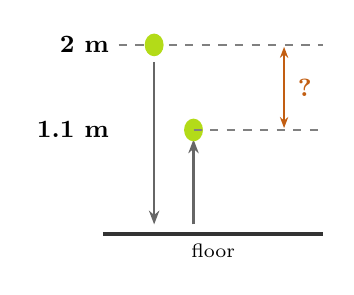
\begin{tikzpicture}[x=1cm, y=1.2cm]
  \draw[black!80, line width=1.4pt] (-0.2,0) -- (2.6,0);
  \node[below, font=\scriptsize] at (1.2,0) {floor};
  \draw[black!50, dashed, line width=0.7pt] (0,2) -- (2.6,2);
  \node[left, font=\small\bfseries] at (0,2) {2 m};
  \fill[yellow!70!green] (0.45,2) circle (0.12);
  \draw[black!60, line width=0.9pt, -{Stealth[length=5pt]}] (0.45,1.82) -- (0.45,0.1);
  \draw[black!60, line width=0.9pt, -{Stealth[length=5pt]}] (0.95,0.1) -- (0.95,1.0);
  \fill[yellow!70!green] (0.95,1.1) circle (0.12);
  \draw[black!50, dashed, line width=0.7pt] (0.95,1.1) -- (2.6,1.1);
  \node[left, font=\small\bfseries] at (0,1.1) {1.1 m};
  \draw[cborange, line width=1pt, {Stealth[length=4pt]}-{Stealth[length=4pt]}]
    (2.1,1.12) -- (2.1,1.98);
  \node[right, font=\small\bfseries, text=cborange] at (2.15,1.55) {?};
\end{tikzpicture}

\vspace{2pt}
\begin{wordhelp}[Word help]
  \small\raggedright
  \eng{How far below 2 m?} = the difference = \textbf{subtract}. \\
  Write 2 as \textbf{2.00}. Or count up to 2: \; $1.6 + 0.4 = 2$.
  \fr{= combien en dessous de 2 m~? = soustraire. \'Ecris 2 sous la forme 2.00, ou
  compte jusqu'\`a 2.}
\end{wordhelp}
\end{minipage}
\end{minipage}

\vspace{8pt}
\noindent\begin{minipage}{\textwidth}
\textbf{(b)} The six bounces were $1.1$, \,$0.05$, \,$1.75$, \,$0$, \,$1.35$ and
$1.5$ m. Write them in order. Start with the \textbf{highest}.
\fr{(b) Range les six rebonds dans l'ordre, du plus haut au plus bas (\eng{start with
the highest}).}

\vspace{8pt}
\noindent\hspace*{1.6em}\blank[1.6cm] \quad \blank[1.6cm] \quad \blank[1.6cm] \quad
\blank[1.6cm] \quad \blank[1.6cm] \quad \blank[1.6cm]
\end{minipage}

\vspace{8pt}
\noindent\begin{minipage}{\textwidth}
\textbf{(c)} At the bounce, some energy changes to \textbf{sound} and \textbf{heat}.
\fr{(c) Au rebond, une partie de l'\'energie devient du son (\eng{sound}) et de la
chaleur (\eng{heat}).}

\vspace{4pt}
\noindent\hspace*{1.6em}Which ball changed the \textbf{most} energy to sound and
heat? \frin{le plus} \hfill \blank[3.2cm] \\[8pt]
\hspace*{1.6em}Which ball changed the \textbf{least}? \frin{le moins} \hfill
\blank[3.2cm]

\vspace{8pt}
\noindent\textbf{(d)} Finish the sentence. \frin{Termine la phrase, en anglais.}
\\[2pt]
\hspace*{1.6em}\eng{The lower the bounce, the more energy \ldots}
\qlines{\frl{2}{3}}
\end{minipage}

% -- X6 ---------------------------------------------------------------------
% The mean of three bounces: an add (three rows) and a divide (the frame).
% (a) has the digits placed; (b) takes them away, and its division frame has
% empty boxes where the total goes.
\qhead[cbgreen]{X6}{Drop it three times}

\begin{remember}[The mean]
  \key{Step 1:} add up all the values. \quad \key{Step 2:} divide by how many there
  are. \quad Three drops: divide by \key{3}.
  \fr{La moyenne (\eng{mean})~: additionne toutes les valeurs, puis divise par le
  nombre de valeurs. Trois l\^achers~: divise par 3.}
\end{remember}

\noindent\begin{minipage}{\textwidth}
\textbf{(a)} The tennis ball bounces \textbf{1.12 m}, \textbf{1.08 m} and
\textbf{1.13 m}. Find the mean.
\fr{(a) La balle de tennis rebondit \`a 1.12 m, 1.08 m et 1.13 m. Calcule la
moyenne.}

\vspace{6pt}
\noindent
\begin{minipage}[t]{0.40\textwidth}\centering
  \textbf{Step 1} \; add\par\vspace{6pt}
  \colgridiii{,1,1,2}{,1,0,8}{,1,1,3}{,,,}
\end{minipage}\hfill
\begin{minipage}[t]{0.30\textwidth}\centering
  \textbf{Step 2} \; $\div\,3$\par\vspace{6pt}
  \bus{3}{3,.,3,3}
\end{minipage}\hfill
\begin{minipage}[t]{0.26\textwidth}\centering
  \vspace{30pt}
  Mean: \blank[1.6cm] m
\end{minipage}
\end{minipage}

\vspace{12pt}
\noindent\begin{minipage}{\textwidth}
\textbf{(b)} The basketball bounces \textbf{1.34 m}, \textbf{1.38 m} and
\textbf{1.36 m}. This time, write the digits in the grid yourself. Then write the
total in the division.
\fr{(b) Le ballon de basket rebondit \`a 1.34 m, 1.38 m et 1.36 m. Cette fois,
\'ecris toi-m\^eme les chiffres dans la grille, puis \'ecris le total dans la
division.}

\vspace{6pt}
\noindent
\begin{minipage}[t]{0.40\textwidth}\centering
  \textbf{Step 1} \; add\par\vspace{6pt}
  \colgridiii{,,,}{,,,}{,,,}{,,,}
\end{minipage}\hfill
\begin{minipage}[t]{0.30\textwidth}\centering
  \textbf{Step 2} \; $\div\,3$\par\vspace{6pt}
  \bus{3}{b,.,b,b}
\end{minipage}\hfill
\begin{minipage}[t]{0.26\textwidth}\centering
  \vspace{30pt}
  Mean: \blank[1.6cm] m
\end{minipage}
\end{minipage}

% -- X7 ---------------------------------------------------------------------
% 3.5's three numbers from the book (page 106). (a) goes through 0.1 litre:
% 40 000 J, so every row is "how many 0.1s?" times 40 000. (b) is partitioning
% (4.5): 2.5 floors = 2 floors + half a floor. (c) divides one by another, as
% the deck's starter did (a kettle in floors of stairs).
\qhead[cbgreen]{X7}{Joules}

\begin{remember}[The book's numbers, from Science 3.5]
  \renewcommand{\arraystretch}{1.2}%
  \begin{tabular}{@{}l@{\quad}l@{\qquad}l@{\quad}l@{\qquad}l@{\quad}l@{}}
    1 floor of stairs: & \key{2\,000 J} & run 1 metre: & \key{200 J} &
    boil 1 litre of water: & \key{400\,000 J} \\
  \end{tabular}
  \fr{Monter 1 \'etage~: 2\,000 J \quad Courir 1 m\`etre~: 200 J \quad Faire bouillir
  1 litre d'eau~: 400\,000 J. Le joule (J) est l'unit\'e de l'\'energie.}
\end{remember}

\noindent\begin{minipage}{\textwidth}
\textbf{(a)} The kettle. $1$ litre needs $400\,000$ J, so $0.1$ litre needs $400\,000
\div 10 = 40\,000$ J. Fill in the table.
\fr{(a) La bouilloire. 1 litre demande 400\,000 J, donc 0.1 litre demande 40\,000 J.
Compl\`ete le tableau.}

\vspace{4pt}
\begin{center}
\begin{tabular}{|C{2.4cm}|C{3.2cm}|C{5.2cm}|}
  \hline
  \textbf{Water (litres)} & \textbf{How many 0.1s?} & \textbf{Energy (J)} \\ \hline
  $0.1$ \tall & $1$ & $1 \times 40\,000 = 40\,000$ \\ \hline
  $0.2$ \tall & $2$ & $2 \times 40\,000 =$ \\ \hline
  $0.5$ \tall & & \\ \hline
  $1.5$ \tall & & \\ \hline
\end{tabular}
\end{center}
\end{minipage}

\vspace{4pt}
\noindent\begin{minipage}{\textwidth}
\textbf{(b)} Split the number. The first one is done for you.
\fr{(b) D\'ecompose le nombre (\eng{split the number}). Le premier est fait pour toi.}

\vspace{6pt}
{\renewcommand{\arraystretch}{1.9}%
\noindent\hspace*{1.6em}\begin{tabular}{@{}l@{\;\;}l@{}}
  Climb $2.5$ floors: & $2$ floors $+$ half a floor $= 4\,000 + 1\,000 =
    \mathbf{5\,000}$ J \\
  Climb $3.5$ floors: & $3$ floors $+$ half a floor $=$ \blank[1.6cm] $+$
    \blank[1.6cm] $=$ \blank[1.8cm] J \\
  Run $12.5$ m: & $12$ m $+$ half a metre $=$ \blank[1.6cm] $+$ \blank[1.6cm] $=$
    \blank[1.8cm] J \\
\end{tabular}}
\end{minipage}

\vspace{8pt}
\noindent\begin{minipage}{\textwidth}
\textbf{(c)} Mr Bowen's cup of tea needs $0.2$ litres of water. How many
\textbf{floors of stairs} could he climb with the energy that boils it? Use your
answer to (a).
\fr{(c) Pour une tasse de th\'e, il faut 0.2 litre d'eau. Combien d'\'etages
(\eng{floors of stairs}) Mr Bowen pourrait-il monter avec l'\'energie qui la fait
bouillir~? Utilise ta r\'eponse au (a).}

\vspace{6pt}
\noindent\hspace*{1.6em}\blank[2.2cm] $\div\ 2\,000 =$ \blank[1.8cm] floors
\end{minipage}

% -- X8 ---------------------------------------------------------------------
% 3.6's write note: thermal energy moves from hotter things to colder things.
% The drops (18.5, 12.5, 8.5) get smaller as the coffee nears the room's
% temperature, and it can never go below it: (d) is the reasoning question.
\qhead[cbgreen]{X8}{Mr Bowen's coffee goes cold}

\noindent\begin{minipage}{\textwidth}
Mr Bowen makes a hot coffee. Then 30 students ask him questions. The room is
\textbf{28.5\,$^{\circ}$C}.
\fr{Mr Bowen se fait un caf\'e chaud. Puis 30 \'el\`eves lui posent des questions.
La salle est \`a 28.5\,$^{\circ}$C.}

\vspace{4pt}
\begin{center}
\begin{tabular}{|l|C{1.7cm}|C{1.7cm}|C{1.7cm}|C{1.7cm}|}
  \hline
  \textbf{Time} (minutes) & $0$ & $10$ & $20$ & $30$ \\ \hline
  \textbf{Coffee} ($^{\circ}$C) & $82.5$ & $64.0$ & $51.5$ & $43.0$ \\ \hline
\end{tabular}
\end{center}

\noindent\textbf{(a)} How much does it cool in each 10 minutes? Subtract. The first
one is done for you.
\fr{(a) De combien refroidit-il toutes les 10 minutes~? Soustrais. Le premier est
fait pour toi.}

\vspace{8pt}
\noindent
\begin{minipage}[t]{0.32\textwidth}\centering
  0 to 10 minutes\par\vspace{6pt}
  \colgrid{-}{8,2,5,}{6,4,0,}{1,8,5,}
\end{minipage}\hfill
\begin{minipage}[t]{0.32\textwidth}\centering
  10 to 20 minutes\par\vspace{6pt}
  \colgrid{-}{6,4,0,}{5,1,5,}{,,,}
\end{minipage}\hfill
\begin{minipage}[t]{0.32\textwidth}\centering
  20 to 30 minutes\par\vspace{6pt}
  \colgrid{-}{,,,}{,,,}{,,,}
\end{minipage}
\end{minipage}

\vspace{10pt}
\noindent\begin{minipage}{\textwidth}
\begin{enumerate}[label=(\alph*), start=2, itemsep=\frl{7pt}{9pt}]
  \item Each 10 minutes, does it cool by \textbf{more} or by \textbf{less}? Circle
        one. \hfill more \qquad less
        \fr{Toutes les 10 minutes, refroidit-il de plus en plus, ou de moins en
        moins~? Entoure (\eng{circle}) une r\'eponse.}
  \item Which way does the \textbf{thermal energy} move? Tick one.
        \fr{Dans quel sens va l'\'energie thermique (\eng{thermal energy})~? Coche une
        case.}
        \par\nobreak\vspace{4pt}
        \tickbox\; from the coffee to the room \frin{du caf\'e vers la salle}
        \qquad \tickbox\; from the room to the coffee \frin{de la salle vers le caf\'e}
  \item Mr Bowen forgets his coffee for 3 hours. Will it get \textbf{colder} than the
        room? Circle one: \; yes \quad no. \; Then explain in a full sentence.
        \; Start: \eng{``Thermal energy only moves from \ldots''}
        \fr{Mr Bowen oublie son caf\'e pendant 3 heures. Sera-t-il plus froid que la
        salle~? Entoure \eng{yes} ou \eng{no}, puis explique par une phrase
        compl\`ete, en anglais.}
        \qlines{\frl{2}{3}}
\end{enumerate}
\end{minipage}

% ===========================================================================
% PART 3 -- SOME ANGLES
% ===========================================================================
\hwsection[cbgreen]{Part 3 \textperiodcentered\ Some angles\frin{Quelques angles}}

\begin{remember}[From Maths 5.1]
  Angles on a \key{straight line} add up to \key{180$^{\circ}$}. \quad Angles
  \key{around a point} add up to \key{360$^{\circ}$}. \\
  \key{Two steps:} \textbf{1.} Add the angles you know. \; \textbf{2.} Subtract the
  total from 180$^{\circ}$ or 360$^{\circ}$.
  \fr{Les angles sur une ligne droite font 180$^{\circ}$ en tout~; autour d'un point,
  360$^{\circ}$. Deux \'etapes~: additionne les angles connus, puis soustrais le total
  de 180$^{\circ}$ ou de 360$^{\circ}$.}
\end{remember}

% -- X9 ---------------------------------------------------------------------
% 3.4's spinning Earth in degrees: 360 in 24 hours is 15 an hour. Six hours is
% a right angle (high tide to low tide), twelve a straight line (high tide to
% high tide), twenty-four a full turn. 0.5 and 2.5 hours are the decimals.
\qhead[cbgreen]{X9}{The Earth turns 15$^{\circ}$ every hour}

\noindent\begin{minipage}{\textwidth}
The Earth spins once a day: $360^{\circ}$ in 24 hours. \; $360 \div 24 = 15$, so it
turns \key{15$^{\circ}$ every hour}. Fill in the table.
\fr{La Terre fait un tour par jour~: 360$^{\circ}$ en 24 heures. $360 \div 24 = 15$~:
elle tourne de 15$^{\circ}$ par heure (\eng{every hour}). Compl\`ete le tableau.}

\vspace{4pt}
{\setlength{\tabcolsep}{5pt}%
\noindent
\begin{tabularx}{\textwidth}{|C{1.5cm}|C{3.2cm}|C{1.9cm}|L|}
  \hline
  \textbf{Hours} & \textbf{Calculation} & \textbf{Degrees} &
  \textbf{At Mr Bowen's harbour} \\ \hline
  $1$ \tall & $1 \times 15$ & $15^{\circ}$ & \\ \hline
  $2$ \tall & $2 \times 15$ & & \\ \hline
  $6$ \tall & & & high tide to low tide: a \blank[2.2cm] angle \\ \hline
  $12$ \tall & & & high tide to high tide: a \blank[2.2cm] line \\ \hline
  $24$ \tall & & & one whole day: a \blank[2.2cm] turn \\ \hline
  $0.5$ \tall & half of 15 & & \\ \hline
  $2.5$ \tall & $30 \,+$ \blank[1.2cm] & & \\ \hline
\end{tabularx}}
\fr{Derni\`ere colonne~: de la mar\'ee haute \`a la mar\'ee basse, un angle \ldots~;
d'une mar\'ee haute \`a la suivante, une ligne \ldots~; un jour entier, un tour
\ldots{} (\eng{right}, \eng{straight}, \eng{full}~: \`a toi de trouver lequel).}
\end{minipage}

% -- X10 --------------------------------------------------------------------
% 360 round a point, cut into equal angles. The turbine is 3.6's wind farm; the
% pizza is 5.1's (8 slices, 45). (b) and (c) start with "will not go": a 0 in
% the first box. (d) halves 45 and runs past the point: 22.5.
\qhead[cbgreen]{X10}{Equal angles around a point}

\noindent\begin{minipage}{\textwidth}
Each one is cut into \textbf{equal} angles. Divide $360^{\circ}$ by how many there
are. Write one digit in each box.
\fr{Chaque objet est partag\'e en angles \'egaux (\eng{equal}). Divise 360$^{\circ}$
par le nombre de parts. \'Ecris un chiffre par case.}

\vspace{8pt}
\noindent
\begin{minipage}[t]{0.24\textwidth}\centering
  \textbf{(a)} A wind turbine:\\ 3 blades \frin{3 pales}\par\vspace{4pt}
  \spokes{3}{90}\par\vspace{6pt}
  \bus{3}{3,6,0}\par\vspace{6pt}
  $=$ \blank[1.2cm]$^{\circ}$
\end{minipage}\hfill
\begin{minipage}[t]{0.24\textwidth}\centering
  \textbf{(b)} A ceiling fan:\\ 5 blades \frin{un ventilateur}\par\vspace{4pt}
  \spokes{5}{90}\par\vspace{6pt}
  \bus{5}{3,6,0}\par\vspace{6pt}
  $=$ \blank[1.2cm]$^{\circ}$
\end{minipage}\hfill
\begin{minipage}[t]{0.24\textwidth}\centering
  \textbf{(c)} A pizza:\\ 8 slices \frin{8 parts}\par\vspace{4pt}
  \spokes{8}{90}\par\vspace{6pt}
  \bus{8}{3,6,0}\par\vspace{6pt}
  $=$ \blank[1.2cm]$^{\circ}$
\end{minipage}\hfill
\begin{minipage}[t]{0.24\textwidth}\centering
  \textbf{(d)} A pizza:\\ 16 slices \frin{16 parts}\par\vspace{4pt}
  \spokes{16}{90}\par\vspace{6pt}
  \bus{2}{4,5,.,z}\par\vspace{6pt}
  $=$ \blank[1.2cm]$^{\circ}$
\end{minipage}

\vspace{6pt}
\noindent\textbf{(d)} needs no new division: a 16-slice slice is \textbf{half} of an
8-slice slice. So it is (c)'s answer $\div\ 2$.
\fr{(d) Pas besoin d'une nouvelle division~: une part sur 16 est la moiti\'e
(\eng{half}) d'une part sur 8. C'est donc la r\'eponse du (c) divis\'ee par 2.}
\end{minipage}

% -- X11 --------------------------------------------------------------------
% 180 on a straight line, with a decimal. (a) is one step, and 180 has to be
% written 180.0. (b) is 3.6's ball rolling down a hill. (c) is the two steps.
\qhead[cbgreen]{X11}{The ramp}

\noindent\begin{minipage}{\textwidth}
\noindent\begin{minipage}[c]{0.46\textwidth}\centering
% The ramp meets the floor at 32.5 degrees (drawn at 32.5).
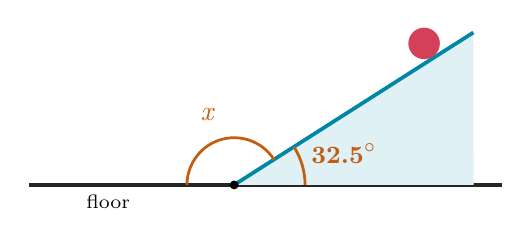
\begin{tikzpicture}[x=1cm, y=1cm]
  \draw[black!85, line width=1.3pt] (-2.6,0) -- (3.4,0);
  \draw[cbteal, line width=1.3pt] (0,0) -- (32.5:3.6);
  \fill[cbteal!12] (0,0) -- (3.04,0) -- (32.5:3.6) -- cycle;
  \draw[cbteal, line width=1.3pt] (0,0) -- (32.5:3.6);
  \fill[cbred!80] ($(32.5:3.0)+(122.5:0.22)$) circle (0.2);
  \draw[cborange, line width=1pt] (0.9,0) arc (0:32.5:0.9);
  \node[font=\small\bfseries, text=cborange] at (16:1.45) {32.5$^{\circ}$};
  \draw[cborange, line width=1pt] (32.5:0.6) arc (32.5:180:0.6);
  \node[font=\bfseries, text=cborange] at (110:0.95) {$x$};
  \fill (0,0) circle (1.6pt);
  \node[below, font=\scriptsize] at (-1.6,0) {floor};
\end{tikzpicture}
\end{minipage}\hfill
\begin{minipage}[c]{0.50\textwidth}
Mr Bowen rolls a ball down a ramp. The ramp makes $32.5^{\circ}$ with the floor.
\fr{Mr Bowen fait rouler une balle sur une rampe (\eng{ramp}). La rampe fait un angle
de 32.5$^{\circ}$ avec le sol.}

\vspace{4pt}
\textbf{(a)} Find $x$. Write $180$ as $180.0$.
\fr{(a) Trouve $x$. \'Ecris 180 sous la forme 180.0.}

\vspace{6pt}
\centering\hgrid{-}{1,8,0,z}{,3,2,5}{,,,}\par\vspace{4pt}
$x =$ \blank[1.6cm]$^{\circ}$
\end{minipage}

\vspace{10pt}
\noindent\textbf{(b)} The ball rolls down. Name the energy change.
\fr{(b) La balle descend la rampe. Nomme le changement d'\'energie.}
\par\nobreak\vspace{6pt}
\noindent\hspace*{1.6em}\blank[4.6cm] \; $\longrightarrow$ \; \blank[4.6cm]
\end{minipage}

\vspace{10pt}
\noindent\begin{minipage}{\textwidth}
\noindent\textbf{(c)} Three angles on a straight line. Find $y$ in two steps.
\fr{(c) Trois angles sur une ligne droite. Trouve $y$ en deux \'etapes.}

\vspace{6pt}
\noindent
\begin{minipage}[t]{0.32\textwidth}\centering
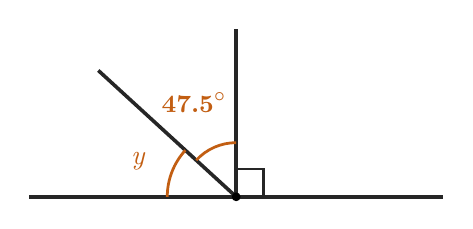
\begin{tikzpicture}[x=1.25cm, y=1.25cm, baseline=(current bounding box.north)]
  \draw[black!85, line width=1.3pt] (-2.1,0) -- (2.1,0);
  \draw[black!85, line width=1.3pt] (0,0) -- (90:1.7);
  \draw[black!85, line width=1.3pt] (0,0) -- (137.5:1.9);
  \draw[black!85, line width=0.9pt] (0.28,0) -- (0.28,0.28) -- (0,0.28);
  \draw[cborange, line width=1pt] (90:0.55) arc (90:137.5:0.55);
  \node[font=\small\bfseries, text=cborange] at (114:1.05) {47.5$^{\circ}$};
  \draw[cborange, line width=1pt] (137.5:0.7) arc (137.5:180:0.7);
  \node[font=\bfseries, text=cborange] at (160:1.05) {$y$};
  \fill (0,0) circle (1.6pt);
\end{tikzpicture}
\end{minipage}\hfill
\begin{minipage}[t]{0.32\textwidth}\centering
  \textbf{Step 1} \; add\par\vspace{6pt}
  \hgrid{+}{,9,0,z}{,4,7,5}{,,,}
\end{minipage}\hfill
\begin{minipage}[t]{0.32\textwidth}\centering
  \textbf{Step 2} \; subtract\par\vspace{6pt}
  \hgrid{-}{1,8,0,z}{,,,}{,,,}
\end{minipage}

\vspace{6pt}
\hspace*{\fill}$y =$ \blank[1.6cm]$^{\circ}$
\end{minipage}

% -- X12 --------------------------------------------------------------------
% The whole sheet in one question: a tidal range (X2), the Earth's turn in
% degrees (X9), a bounce (X5) and where its energy went (3.6), and a store
% (3.5). Last on purpose.
\qhead[cbgreen]{X12}{The whole sheet in one question}

\noindent\begin{minipage}{\textwidth}
Mr Bowen spends a day at the beach. High tide is \textbf{4.6 m} at \textbf{7 a.m.}
Low tide is \textbf{0.75 m} at \textbf{1 p.m.}
\fr{Mr Bowen passe la journ\'ee \`a la plage. Mar\'ee haute~: 4.6 m \`a 7 h du matin
(\eng{7 a.m.}). Mar\'ee basse~: 0.75 m \`a 13 h (\eng{1 p.m.}).}

\vspace{6pt}
\noindent\begin{minipage}[t]{0.62\textwidth}
\textbf{(a)} What is the \textbf{tidal range}?
\fr{(a) Quel est le marnage (\eng{tidal range})~?}

\vspace{4pt}
\hspace*{1.6em}Tidal range: \blank[1.8cm] m

\vspace{10pt}
\textbf{(b)} From high tide to low tide is \blank[1.0cm] hours.
\fr{(b) De la mar\'ee haute \`a la mar\'ee basse, il y a \ldots{} heures.}

\vspace{4pt}
\hspace*{1.6em}The Earth turns \blank[1.0cm] $\times\ 15 =$
\blank[1.4cm]$^{\circ}$. \\[6pt]
\hspace*{1.6em}That is a \blank[2.6cm] angle.
\fr{La Terre tourne de \ldots{} degr\'es~: quel type d'angle (\eng{angle})~?}
\end{minipage}\hfill
\begin{minipage}[t]{0.34\textwidth}\centering
  \vspace{0pt}
  \colgrid{-}{,4,6,z}{,0,7,5}{,,,}
\end{minipage}
\end{minipage}

\vspace{10pt}
\noindent\begin{minipage}{\textwidth}
\noindent\begin{minipage}[t]{0.62\textwidth}
\textbf{(c)} Mr Bowen drops a ball from \textbf{2 m} onto the sand. It bounces only
\textbf{0.35 m}. How far below 2 m does it stop?
\fr{(c) Mr Bowen l\^ache une balle de 2 m sur le sable. Elle ne rebondit qu'\`a 0.35
m. \`A combien en dessous de 2 m s'arr\^ete-t-elle~?}

\vspace{4pt}
\hspace*{1.6em}\blank[1.8cm] m

\vspace{10pt}
\textbf{(d)} In his hand, what energy store does the ball have?
\fr{(d) Dans sa main, quelle r\'eserve d'\'energie (\eng{energy store}) la balle
a-t-elle~?}

\vspace{4pt}
\hspace*{1.6em}\blank[5.4cm]
\end{minipage}\hfill
\begin{minipage}[t]{0.34\textwidth}\centering
  \vspace{0pt}
  \colgrid{-}{,2,z,z}{,0,3,5}{,,,}
\end{minipage}
\end{minipage}

\vspace{10pt}
\noindent\begin{minipage}{\textwidth}
\textbf{(e)} The ball did not come back to 2 m. Where did the rest of its energy go?
Answer in a full sentence. \; Start: \eng{``When the ball hit the sand, \ldots''}
\fr{(e) La balle n'est pas remont\'ee \`a 2 m. O\`u est partie le reste de son
\'energie~? R\'eponds par une phrase compl\`ete, en anglais.}
\qlines{\frl{5}{4}}
\end{minipage}

% ===========================================================================
% ANSWER KEY -- TEACHER COPY ONLY
% ===========================================================================
\ifkey
\clearpage

\hwsection[cbred]{Answer Key --- Teacher Copy}

\linespread{1.0}\selectfont
\setlist[enumerate]{itemsep=2pt, topsep=3pt, leftmargin=*}
\setlist[itemize]{itemsep=2pt, topsep=3pt, leftmargin=*}

\qhead[cbred]{X1}{Read the tide board}
\noindent (a) 4 a.m. $5.4$ \sep 6 a.m. $4.4$ \sep 8 a.m. $2.2$ \sep 10 a.m. $1.2$ m \quad
(b) 4 a.m. \quad (c) 10 a.m.

\smallskip
\noindent{\small Each small line is $0.2$, not $0.1$. A student who counts ticks as
tenths writes $5.2$, $4.2$, $2.1$, $1.1$: every reading half as far above the metre
line. The remedy is the sheet's own line: count in 0.2s, 5, 5.2, 5.4.}

\qhead[cbred]{X2}{The tidal range}
\noindent (b) $3.75 - 0.90 = 2.85$ m \quad (c) $6.10 - 2.35 = 3.75$ m \quad (d) $16.3
- 4.2 = 12.1$ m

\smallskip
\noindent{\small (b) and (c) are the orange-box zeros. Taking the smaller digit from
the bigger in each column gives $3.25$ for (b) and $4.25$ for (c): the student has
not borrowed. \\
(d) has no digits printed: the student places $16.3$ and $4.2$ in the grid. Both
have one decimal place, so a wrongly placed grid can still give $12.1$; check the
grid, not only the answer.}

\qhead[cbred]{X3}{Half above, half below}
\noindent
\begin{tabular}{@{}lllll@{}}
  $4.5$, $3.0$: & half $1.5$ & deepest $6.0$ & shallowest $3.0$ \\
  $3.2$, $1.4$: & half $0.7$ & deepest $3.9$ & shallowest $2.5$ \\
  $6.0$, $2.5$: & half $1.25$ & deepest $7.25$ & shallowest $4.75$ \\
\end{tabular} \\
(b) \emph{He added the whole range to the average. He should add half of it: $4.5 +
1.5 = 6.0$ m.}

\smallskip
\noindent{\small The book's Question 6 (3.4), the trap the deck called out: the range
is the \emph{whole} distance from low to high. \\
Row 4 runs past the point: $2.5 \div 2 = 1.25$. Expect $1.2$ or $1.3$ from a student
who stops at one decimal place, and then $7.2$ and $4.8$.}

\qhead[cbred]{X4}{The land has tides too}
\noindent (a) $0.3$ m \quad (b) $0.6$ m \quad (c) $42$, \ $4.2$ m \\
(d) \emph{We do not feel it because everything goes up and down together: the
ground, the buildings and us.}

\smallskip
\noindent{\small (a) Expect $3$ or $0.03$: the point moved one place too few or one
too many. $30 \div 100$: two places left. \\
(c) $4.2$ m in a week, and nobody noticed: that is the joke, and (d) is why.}

\qhead[cbred]{X5}{Six balls, one floor}
\noindent (a) clay $1.95$ \sep bouncy ball $0.25$ \sep egg $2$ ($2.00$) \sep basketball
$0.65$ \sep ping-pong $0.50$ \\
(b) $1.75$, \ $1.5$, \ $1.35$, \ $1.1$, \ $0.05$, \ $0$ \\
(c) most: the egg (accept the clay) \sep least: the bouncy ball \\
(d) \emph{The lower the bounce, the more energy changed to sound and heat at the
floor.}

\smallskip
\noindent{\small (a) is ``write 2 as 2.00''. An answer that starts with 1 ($1.25$ for
the bouncy ball, $1.65$ for the basketball) did not borrow from the 2. Counting up is
the check: $1.75 + 0.25 = 2$. \\
(b) $1.5 > 1.35$ is the Unit 4 trap (the shorter number is bigger: $1.50$). A list
with $1.35$ before $1.5$ has compared the digit count. \\
(c) The egg and the clay both stop dead; either is right. The point is the
direction: a \emph{low} bounce means \emph{more} energy left the ball.}

\qhead[cbred]{X6}{Drop it three times}
\noindent (a) $1.12 + 1.08 + 1.13 = 3.33$; \ $3.33 \div 3 = \mathbf{1.11}$ m \quad
(b) $1.34 + 1.38 + 1.36 = 4.08$; \ $4.08 \div 3 = \mathbf{1.36}$ m

\smallskip
\noindent{\small (b) has a 0 in the total. $4 \div 3 = 1$ r 1, then $10 \div 3 = 3$ r
1, then $18 \div 3 = 6$. A student who drops the 0 divides $4.8$ and gets $1.6$ ---
bigger than every bounce, which is the check: a mean sits \emph{between} the
values.}

\qhead[cbred]{X7}{Joules}
\noindent (a) $0.2$: $80\,000$ \sep $0.5$: $5 \times 40\,000 = 200\,000$ \sep $1.5$: $15
\times 40\,000 = 600\,000$ J \\
(b) $3.5$ floors: $6\,000 + 1\,000 = 7\,000$ J \sep $12.5$ m: $2\,400 + 100 = 2\,500$ J
\\
(c) $80\,000 \div 2\,000 = 40$ floors

\smallskip
\noindent{\small (a) ``How many 0.1s in 1.5?'' is 15. Expect 5 (the digit after the
point) or 1.5 (copied). \\
(b) Half a metre of running is $100$ J; expect $200$ from a student who reads
``half a metre'' as ``a metre''. \\
(c) is the deck's starter in small: the kettle in floors of stairs (there, 200
floors for a litre).}

\qhead[cbred]{X8}{Mr Bowen's coffee goes cold}
\noindent (a) $64.0 - 51.5 = 12.5$ \sep $51.5 - 43.0 = 8.5$ \quad (b) less \quad (c) from
the coffee to the room \\
(d) \textbf{no}. \emph{Thermal energy only moves from hotter things to colder things,
so the coffee stops cooling when it is as warm as the room (28.5\,$^{\circ}$C).}

\smallskip
\noindent{\small (a) $64.0 - 51.5$: expect $13.5$, the smaller digit taken from the
bigger in the tenths ($5 - 0$) instead of borrowing. \\
(d) is the reasoning question: the write note says which way heat moves, so once the
coffee is at room temperature there is nowhere colder for it to go. ``Yes, it keeps
getting colder'' has read the drops (18.5, 12.5, 8.5) as if they never stop.}

\qhead[cbred]{X9}{The Earth turns 15\textdegree\ every hour}
\noindent 2 h $30^{\circ}$ \sep 6 h $90^{\circ}$, a \textbf{right} angle \sep 12 h
$180^{\circ}$, a \textbf{straight} line \sep 24 h $360^{\circ}$, a \textbf{full} turn
\sep 0.5 h $7.5^{\circ}$ \sep 2.5 h $30 + 7.5 = 37.5^{\circ}$

\smallskip
\noindent{\small Homework 11's F1 is this table's reason: the two bulges are
$180^{\circ}$ apart, so high tide comes every 12 hours. \\
$0.5 \times 15$: expect $7$ or $8$ from a student who will not write a decimal angle.}

\qhead[cbred]{X10}{Equal angles around a point}
\noindent (a) $120^{\circ}$ \sep (b) $72^{\circ}$ \sep (c) $45^{\circ}$ \sep (d) $45.0
\div 2 = 22.5^{\circ}$

\smallskip
\noindent{\small (b) and (c): 5 and 8 will not go into 3, so the first answer box is
0 ($072$, $045$). A student who leaves the box empty and slides the digits left
writes $720$ or $450$. \\
(d) runs past the point into the orange box: $45.0$.}

\qhead[cbred]{X11}{The ramp}
\noindent (a) $180.0 - 32.5 = 147.5^{\circ}$ \quad (b) gravitational potential
$\to$ kinetic \quad (c) $90 + 47.5 = 137.5$; \ $180 - 137.5 = 42.5^{\circ}$

\smallskip
\noindent{\small (a) Expect $152.5$: the smaller digit taken from the bigger in the
tenths and the ones, with no borrowing. The orange 0 is there to make the borrow
visible. \\
(c) The small square is $90^{\circ}$ and is not written as a number: expect
$132.5^{\circ}$ ($180 - 47.5$) from a student who missed it.}

\qhead[cbred]{X12}{The whole sheet in one question}
\noindent (a) $4.60 - 0.75 = 3.85$ m \quad (b) 6 hours; \ $6 \times 15 = 90^{\circ}$; a
right angle \quad (c) $2.00 - 0.35 = 1.65$ m \\
(d) gravitational potential \\
(e) \emph{When the ball hit the sand, some of its energy changed to sound and heat,
so it could not lift the ball back up to 2 m.}

\smallskip
\noindent{\small (a) $4.6$ needs its orange 0: expect $4.15$ without it. \\
(e) ``The sand is soft'' is true and is not the answer; ask where the energy
\emph{went}.}

\fi

\end{document}
